% !TEX root =../articulo.tex
\section{El algoritmo CUSUM}\label{sec:CUSUM}

\subsection{Control de procesos}
El objetivo del \gls{CdP} es el de establecer un sistema de observación permanente e inteligente,
que detecte la aparición de variabilidad sobre la norma de un parámetro e identifique su origen, de forma que 
sea posible evitar su reaparición \cite{Control_de_procesos}. %TODO: ¿debería definirse antes el algoritmo CUSUM? Queda raro y hasta leer el siguiente epígrafe no se entiende la relación con el título de la sección. Quizá la definición del CdP podría ir simplemente como una nota al pie. 

\subsection{Algoritmo CUSUM}
El algoritmo CUSUM es un sistema de \gls{CdP} con memoria, es decir, la salida del
sistema no solo depende del estado actual de la variable de control, sino también del
estado anterior de la misma. De esta forma, restamos importancia a las desviaciones 
puntuales de la variable, y al mismo tiempo logramos resaltar los cambios pequeños
pero prolongados en el tiempo \cite{CUSUM_Carlos_III}.

Ante una Variable de Interés $x_i$, que sigue una distribución normal 
$x_i \sim\mathcal{N}\left(\mu_0,\sigma^2\right)$, 
construimos el estadístico $C_i$ que acumula la desviación de la variable sobre su media
a lo largo de las muestras:
\begin{align*}
 C_1 &= (x_1 - \mu_0) \nonumber\\
 C_2 &= (x_1 - \mu_0) + (x_1 - \mu_0) = C_1 + (x_2-\mu_0) \nonumber\\
 &\vdots& \nonumber\\
 C_i &= C_{i-1} + (x_i-\mu_0)
\end{align*}

\begin{figure}[htbp]
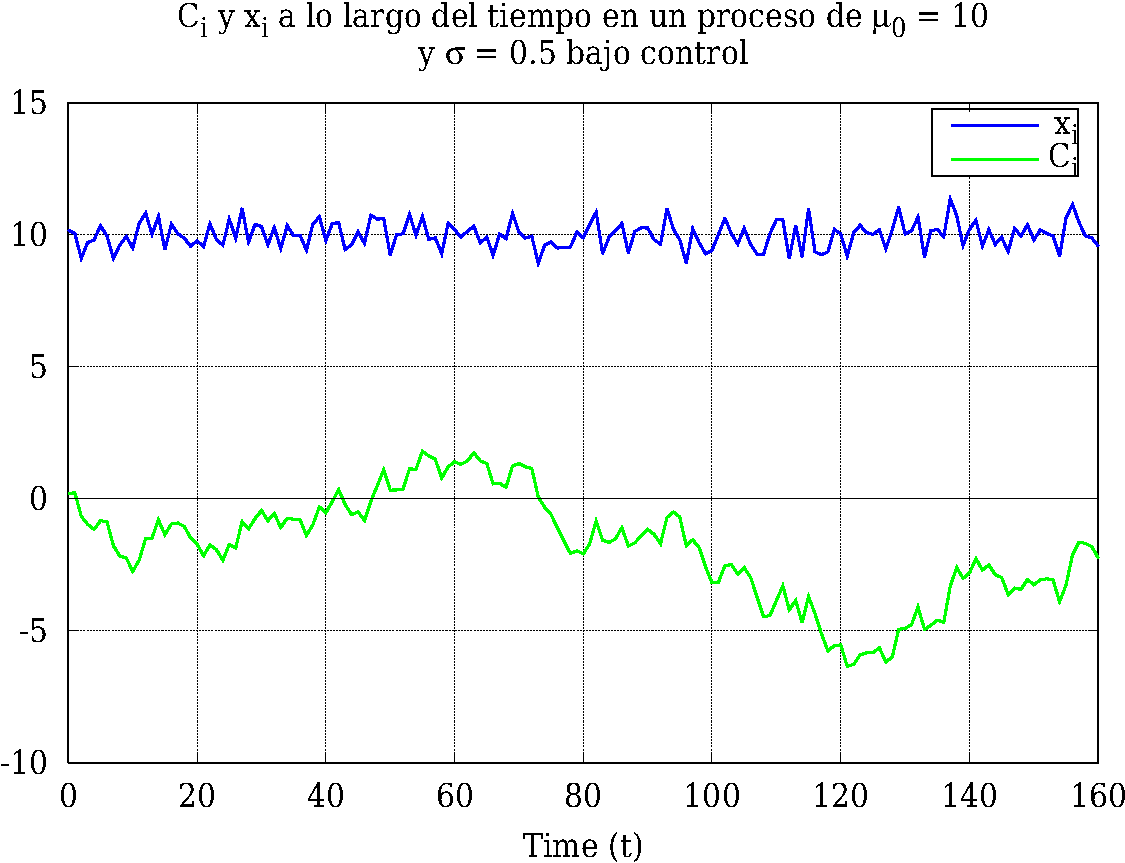
\includegraphics[width=\columnwidth]{CapituloCusum/Figuras/ejemploCusumControlado_crop}
\caption{Algoritmo CUSUM aplicado sobre un proceso controlado}
\label{fig:cusum_controlado} 
\end{figure}

\begin{figure}[htbp]
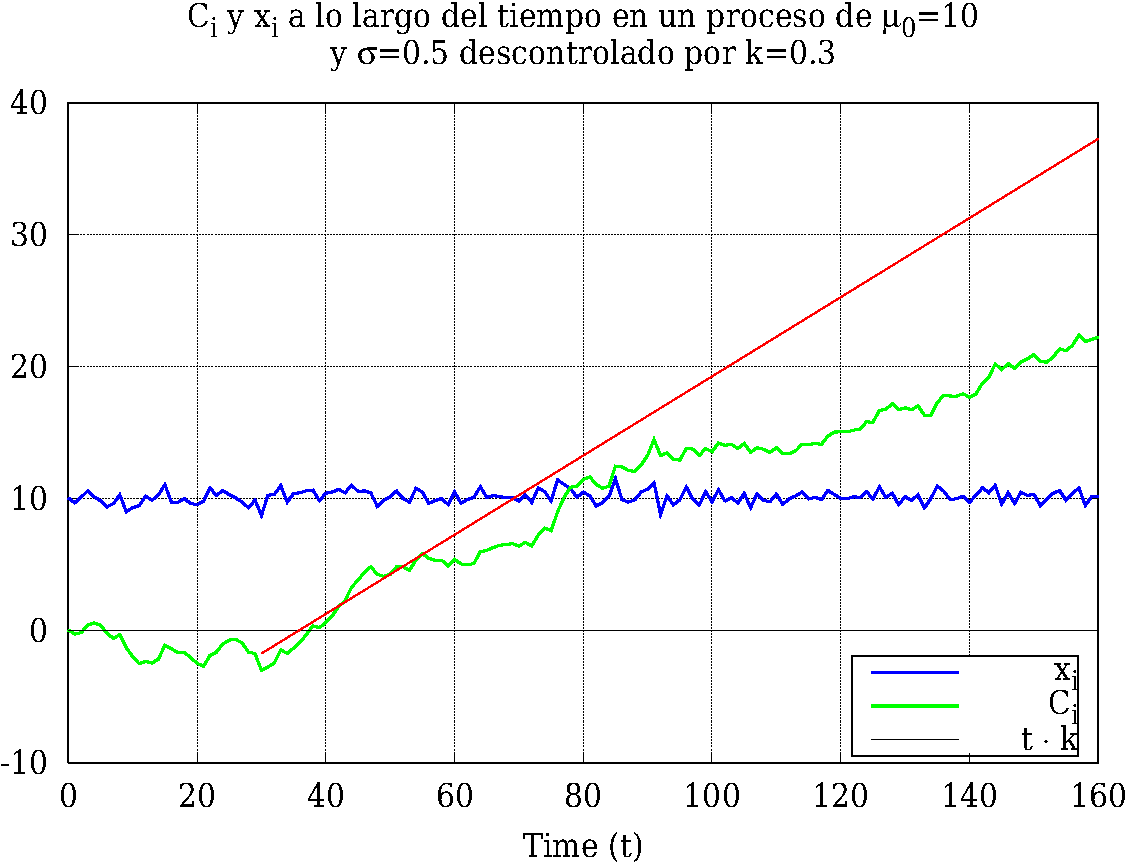
\includegraphics[width=\columnwidth]{CapituloCusum/Figuras/cusumDescontrolado-crop}
\caption{Algoritmo CUSUM aplicado sobre un proceso perturbado}
\label{fig:cusum_descontrolado} 
\end{figure}

Esto es, si las distintas muestras oscilan alrededor de $\mu_0$, $C_i$ tenderá a valer 0, %TODO me suena rara esta expresión. Tenderá a ser igual a 0.
como vemos en \autoref{fig:cusum_controlado}. Por su parte, si las muestras presentan 
una desviación $k$ sobre $mu_0$, $C_i$ seguirá una recta $C_i=ik$ de pendiente $k$, 
como vemos en la \autoref{fig:cusum_descontrolado}. De esta forma, podemos definir una
variable descontrolada como aquella cuyo parámetro
$C_i$ ha superado un umbral definido para esa variable (normalmente, en forma de un
umbral de sensibilidad $C_i^+=M\sigma$).

Si queremos que las pequeñas variaciones no afecten al algoritmo, es posible también
definir un umbral mínimo sobre la desviación de la media $C_i^{min}=m\sigma$, de 
forma que sólo sumemos a $C_i$ las desviaciones superiores a $C_i^{min}$.

\subsection{Algoritmo CUSUM aplicado al control del tráfico}
\label{ssec:cusum_aplicado_trafico}
El tráfico de red es un proceso especialmente caótico, tanto por el número de posibles
parámetros a controlar como por la alta variabilidad de éstos,
haciendo imposible definir un valor ``normal'' para éstos, tal y como se señaló en la 
\autoref{sssec:ddos_deteccion_inundacion}.

S.V. Raghvan y E.Dawson establecen como parámetros más importantes a la hora de detectar un ataque 
\gls{DoS} los siguientes:

% TODO Quizás deberíamos decir: Todos en relación al número de paquetes IP excepto X, Y, Z?

\begin{enumerate}
 \item \gls{OWCD}, Densidad de conexiones de un solo sentido
 \begin{align*}
  \text{OWCD} = \frac{\sum\text{Paquetes OWC}}{\sum\text{Paquetes IP}}
 \end{align*}

 \item Longitud media de paquetes: 
   $\langle L\rangle_{\text{flow}} = \frac{\sum\text{Long paquetes IP}}{\sum\text{Paquetes IP}}$
 
 \item Relación entre paquetes entrantes y salientes: 
   $\frac{\sum\text{Paquetes entrantes}}{\sum\text{Paquetes salientes}}$
 
 \item \% de paquetes TCP: $\frac{\sum\text{Paquetes TCP}}{\sum\text{Paquetes IP}}$ 
 \item \% de paquetes UDP: $\frac{\sum\text{Paquetes UDP}}{\sum\text{Paquetes IP}}$
 \item Paquetes ICMP: $\frac{\sum\text{Paquetes ICMP}}{\sum\text{Paquetes IP}}$
 \item \% de paquetes LAND\footnote{Misma dirección origen y destino.}.
 \item Protocolo capa 4.
\end{enumerate}

\subsection{Algoritmo propuesto}
\begin{figure}[htbp]
\centering
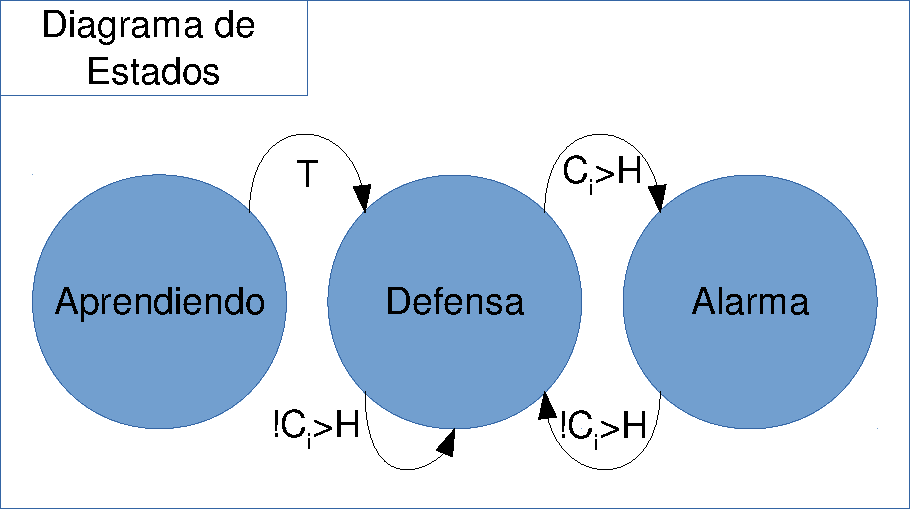
\includegraphics[width=0.8\columnwidth]{CapituloCusum/Figuras/DiagramaEstados-crop}
\caption{Diagrama de estados del sensor}
\label{fig:diagrama_estados} 
\end{figure}

El sistema de defensa \redborderddos monitoriza periódicamente estos parámetros
para cada dirección IP externa a la red y para el tráfico normal que atraviesa
la misma. El sistema podrá encontrarse en tres estados distintos, que se ven reflejados
en la \autoref{fig:diagrama_estados}.

El primero de ellos es el de \textbf{aprendizaje:} al
inicio del programa y durante un tiempo determinado\footnote{Definir dicho
periodo es importante para la precisión de la media obtenida, ya que, por ejemplo, incluso en
verano o en invierno se pueden observar diferencias en una red corporativa.}
el sistema averiguará los parámetros de los estadísticos descritos en la 
\autoref{ssec:cusum_aplicado_trafico}. Es importante que no ocurra ningún
ataque durante este periodo, ya que en ese caso el sistema tomará como normales
los valores de los resultados estadísticos bajo ataque. %TODO: para mayor claridad haría listado con viñetas (Aprendizaje/ Defensa) o destacaría en negrita. 

El segundo estado es el de \textbf{defensa:} durante un periodo determinado, el programa comparará
los parámetros en tiempo real contra la media obtenida en el anterior periodo y
unos parámetros de desviación $C_i^+$ y $C_i^{min}$ especificados en forma de múltiplos
de la desviación típica obtenida. Si durante este periodo no se detecta ningún ataque, los nuevos
valores $\mu_0$ y $\sigma$ obtenidos para cada resultado estadístico pasarán a ser los estándares, de
forma que las variaciones normales no cuenten como un ataque. En caso contrario, el sistema pasará al modo alerta en el mismo
momento que un estadístico supera su umbral. %Revisar el uso de la palabra estadístico. 

Por último, tenemos el estado de \textbf{alerta,} al que se pasará cuando algún parámetro supere su umbral. Este estado finaliza en el
momento en el que los parámetros vuelven a la normalidad. En este caso, se bloqueará el tráfico desde
las direcciones IP detectadas, y sólo cuando el parámetro vuelva a estar bajo el límite\footnote{Teniendo
en cuenta el tráfico bloqueado en el conteo de estadísticos.} se volverá al modo defensa.

\endinput
